\chapter{Background}\label{sec:background}
This section offers a brief introduction on some key notions required to understand the rest of this document.
We start off by looking into formal languages and associated definitions in \autoref{sec:languages}, where we also define regular expressions, one of the main goals of our synthesis procedure\footnote{Definitions and examples in \autoref{sec:languages}
were, in part, adapted from Chapter~3 of \textit{Compilers: Principles, Techniques, and Tools}, by \citet*{DragonBook}.}.
\todo{Section about logic \autoref{sec:logic}.\footnote{Definitions and examples in \autoref{sec:logic}
were, in part, adapted from \textit{Handbook of Satisfiability}, by \citet*{HandbookSAT}.}}
Finally, in \autoref{sec:ps}, we present an overview of the basic concepts of program synthesis.

\section{Regular Languages}\label{sec:languages}
Formal languages differ from the common meaning of the word \textit{language} in that they are built from a set of well-defined rules and thus stringently specified. Programming languages, such as \texttt{C} or \texttt{Python}, are examples of formal languages. They have a strict syntax and no deviation is tolerated: if a string does not comply with the syntax rules, it is not in the language.

To define a formal language, we must first define an alphabet.
An alphabet is a nonempty finite set whose elements are called the symbols, letters or tokens.
Symbols of the alphabet can be, for example, letters, digits, or punctuation marks. Alphabets are usually identified by capital Greek letters.

\begin{definition}[Alphabet]
An alphabet \(\Sigma\) is a nonempty finite set of symbols.
\end{definition}

\begin{example}
The following are examples of alphabets:

\begin{itemize}[topsep=0pt]
\item \(\Sigma_1 = \{0,1\}\): the binary alphabet,
\item \(\Sigma_2 = \{a,b,c,d,e,f,g,h,i,j,k,l,m,n,o,p,q,r,s,t,u,v,w,x,y,z\}\): the Latin lowercase alphabet.
\end{itemize}
\end{example}

Typically, the alphabets used in programming applications are larger than \(\Sigma_1\) or \(\Sigma_2\). The ASCII alphabet, for instance, contains 128 symbols which include all non-accentuated upper- and lower-case letters, digits, and most punctuation marks.

Given an alphabet, we can define strings (also called sentences or words) over it, which result from the concatenation of a finite number of the alphabet's symbols. Strings are usually identified by lower case letters and written between single quotes. The length of a string \(s\), denoted \(|s|\), is the number of symbols in it.

\begin{definition}[String]
A string \(s\) over an alphabet \(\Sigma\) is a finite sequence of symbols drawn from \(\Sigma\).
\end{definition}

\begin{definition}[Length of a string]
The length of a string \(s\), \(|s|\), is the number of symbols in \(s\).
\end{definition}

\begin{example}
The following are examples of strings:
\begin{itemize}[nosep]
\item \(\epsilon\), the empty string, is the string of length zero,\par
\item \(s_1 = \) \textit{synthesis} is a string over alphabet \(\Sigma_2\) and it has length \(|s_1| = 9\).
\end{itemize}
\end{example}

At last, a language is a (finite or infinite) countable set of strings over some alphabet. Languages are usually identified by calligraphic capital letters.

\begin{definition}[Language]
A language \(\mathcal{L}\) is a countable set of strings over some fixed alphabet \(\Sigma\).
\end{definition}

\begin{example}
The following are examples of languages:
\begin{itemize}[nosep]
\item \(\emptyset\), the empty set, is a language which contains no strings,\par
\item \{\(\epsilon\)\} is the language that contains only the empty string.
\end{itemize}
\end{example}

\subsection{Regular Operations}
Regular operations are a type of operation over languages, and regular languages are a subset of languages that are closed under regular operations. The three most basic regular operations are union, concatenation and closure.

The union of two languages \(\mathcal{L}\) and \(\mathcal{M}\), denoted \(\mathcal{L} \cup \mathcal{M}\), is the set of all strings in \(\mathcal{L}\) and all strings in \(\mathcal{M}\) (including those that are in both).
The concatenation of two languages \(\mathcal{L}\) and \(\mathcal{M}\), denoted \(\mathcal{L}\mathcal{M}\), is the set all strings formed by taking any string from \(\mathcal{L}\) and any string from \(\mathcal{M}\) and concatenating them. The concatenation of the same language, \(\mathcal{L}\), \(n\) times is sometimes denoted as \(\mathcal{L}^n\). For example  \(\mathcal{L}^3 = \mathcal{L}\mathcal{L}\mathcal{L}\).
The Kleene closure\footnotemark{} (also called Kleene star or simply star) of a language \(\mathcal{L}\), denoted \(\mathcal{L}^*\), is the set of strings resulting from the concatenation of any string in \(\mathcal{L}\) zero or more times. The Kleene closure of any language always includes the empty string.

\footnotetext{Kleene closure owes its name to the American mathematician Stephen Cole Kleene, who first described the concepts of regular language and regular expression in the~1950s.}
\begin{definition}[Regular operations] There are 3 regular operations on languages, union, concatenation and closure, which are defined as follows:
\begin{itemize}[nosep]
\item Union: \(\mathcal{L} \cup \mathcal{M} = \{s :s \in \mathcal{L}\) \text{ or } \(s \in \mathcal{M}\}\),

\item Concatenation: \(\mathcal{L}\mathcal{M} =\{st : s \in \mathcal{L} \text{ and } t \in \mathcal{M}\}\),

\item Kleene closure: \(\mathcal{L}^*\) = \(\bigcup_{i=0}^\infty \mathcal{L}^i\).
\end{itemize}
\end{definition}

\subsection{Regular Expressions} \label{sec:regex}
Regular expressions are used to describe regular languages. The language defined by a regular expression \(r\) is represented as \(\mathcal{L}(r)\).
Regular expressions are built recursively out of smaller regular expressions connected by operators. The simplest regular expressions refer to languages that contain just one symbol and are represented as that symbol in monospaced font.

\begin{example}
The regular expression \regex{a} defines the language \(\mathcal{L}({\regexm{a}}) =\) \{\textit{a}\}.
\end{example}{}

\begin{table}[t]
\centering

\newcolumntype{R}{>{\arraybackslash}m{.18\textwidth}}
\newcolumntype{L}{>{\arraybackslash}m{.2\textwidth}}
\newcolumntype{M}{>{\arraybackslash}m{.15\textwidth}}
\setlength\extrarowheight{.5em}

\begin{tabular}{l c c}
\toprule
Name & \makecell{Operation on\\regular expressions} & \makecell{Operation on\\languages} \\ \midrule
Union          & \(r|q\) & \quad \(\mathcal{L}(r) \cup \mathcal{L}(q)\) \\
Concatenation  & \(rq\)  & \quad \(\mathcal{L}(r)\mathcal{L}(q)\) \\
Kleene closure & \(r^*\) & \quad \(\mathcal{L}(r)^*\)\\
%  &  Positive closure of \(\mathcal{L}\)                  & \quad \(\mathcal{L}^*\) = \(\cup_{i=1}^\infty \mathcal{L}^i\)                                                           \\ 
\bottomrule
\end{tabular}
\caption{Regular operations}
\label{tab:regex-ops}
\end{table}


All regular operations have a counterpart operation on regular expressions. For example, the union of two regular expressions \(r\) and \(q\) results in a regular expression that defines the regular language \(\mathcal{L}(r) \cup \mathcal{L}(q)\). 
Since regular languages are closed under regular operations, it is possible to apply these operations to any regular expression.
The operations in regular expressions are generally represented in the same way as their regular-language counterparts, with the exception of union, which is represented using a \(|\) instead of the usual set notation~\(\cup\). The operations on regular expressions and their equivalent regular operations  are defined in \autoref{tab:regex-ops}.

The unary operator * has highest precedence, concatenation has second highest precedence and operator \(|\) has lowest precedence.
All three operators are left associative. Parentheses can be used to ensure a subexpression takes precedence over the rest.

\begin{example}
\regex{a|b*c} is a regular expression that defines the language
\[\mathcal{L}(\regexm{a|b*c}) = \{a\} \cup \{b\}^* \{c\}\]
over the alphabet \(\Sigma = \{a, b, c\}\). This language contains strings that are either a single \(a\) or zero or more \(b\)s followed by one \(c\).
\end{example}

If two regular expressions \(r\) and \(s\) denote the same regular language, we say they are equivalent and write \(r = s\). For instance, \regex{a|b} = \regex{b|a}. % There are several algebraic laws that hold for arbitrary regular expressions, some of which are defined in \autoref{tab:regex-laws}.

% \begin{table}[t]
\centering
\begin{tabular}{@{}c c@{}}
\toprule
Algebraic Law                      & \quad Description                                    \\ \midrule
\(r|s = s|r\)                      & \quad Union is commutative                           \\
\(r|(s|t) = (r|s)|t\)              & \quad Union is associative                           \\
\(r(st) = (rs)t\)                  & \quad Concatenation is associative                   \\
\(r(s|t) = rs|rt; (s|t)r = sr|tr\) & \quad Concatenations distributes over union          \\ 
%\(\epsilon r = r\epsilon = r\)     & \quad \(\epsilon\) is the identity for concatenation \\ 
%\(r^* = (r|\epsilon)^*\)           & \quad \(\epsilon\) is guaranteed in a Kleene closure \\ 
\(r|r = r\)      & \quad Union is idempotent \\
\(r^{**} = r^*\)   & \quad * is idempotent \\
\(r?? = r?\)       & \quad ? is idempotent \\
\(r^{++} = r^+\)   & \quad + is idempotent \\

\(r^{+*} = r^{*+} = r^*\)  & \quad .......... \\
\(r?^* = r^*? = r^*\)      & \quad .......... \\
\(r?^+ = r^+? = r^*\)      & \quad .......... \\ \bottomrule
\end{tabular}
\caption{Algebraic laws for regular expression operators}
\label{tab:regex-laws}
\end{table}

\medskip
Since the introduction of regular expressions with the basic operators for union, concatenation, and Kleene closure, some new operators have been defined for regular expressions with the purpose of easing the specification of certain string patterns. Here we show three of those commonly used operators: \(+\), \(?\), and character classes.

The unary postfix operator \(+\) represents positive closure, which can be interpreted as `one or more occurrences of' (note the similarity to Kleene closure, `zero or more instances of'). It can be defined as
\[r^+ = rr^* = r^*r,\]
and gives rise to a new algebraic law:
\[r^* = r^+|\epsilon.\]
%
The unary postfix operator \(?\) means `zero or one
occurrences of', and can be defined~as
\[ r? = r|\epsilon. \]
%
The operators \(+\) and \(?\) have the same precedence and associativity as operator~\(*\).


Character classes are a form of regular expression shorthand notation. A regular expression \(a_1|a_2|a_3|...|a_n\), where each \(a_i\) is a symbol of the alphabet, can be replaced by the shorthand \([a_1 a_2...a_n]\).
When \(a_1 a_2...a_n\) form a logical sequence, e.g., consecutive uppercase letters, lowercase letters, or digits, we
can replace them by \(a_1\mhyphen a_n\), that is, just the first and last tokens separated by
a hyphen.

%\mathchardef\mhyphen="2D

\begin{example}
The following are examples of character classes:
\begin{itemize}[]
\setlength\itemsep{1em}
\item \regex{[abc]} = \regex{a|b|c}
\item \regex{[a\mhyphen z]} = \regex{a|b|...|z}
\item \regex{[a\mhyphen z0\mhyphen 9]} = \regex{a|b|...|z|0|1|...|9}
\end{itemize}
\end{example}

\begin{comment}

\subsection{Regular Definitions}

For convenience, we may wish to give names to certain regular expressions and use those names in subsequent expressions, as if the names were themselves symbols. If \(\Sigma\) is an alphabet of basic symbols, then a regular definition is a sequence of definitions of the form:

\begin{equation}
\begin{gathered} % centered multiline equation.
d_1 \to r_1\\
d_2 \to r_2\\
...\\
d_n \to r_n
\end{gathered}
\end{equation}

\noindent
where each \(d_i\) is a new symbol, not in \(\Sigma\) and not the same as any of the other \(d\), and each \(r_i\) is a regular expression over the alphabet \(\Sigma \cup \{ d_1, d_2, ..., d_{i-1} \}\).

By restricting \(r_i\) to \(\Sigma\) and the previously defined \(d\)'s, we avoid recursive definitions, and we can construct a regular expression over \(\Sigma\) alone, for each \(r_i\).
We do so by first replacing uses of \(d_1\) in \(r_2\) (which cannot use any of the d's except
for \(d_1\)), then replacing uses of \(d_1\) and \(d_2\) in \(r_3\) by \(r_1\) and (the substituted) \(r_2\), and so on. Finally, in \(r_n\) we replace each \(d_i\), for \(i = 1, 2, ..., n-1\), by the substituted version of \(r_i\), each of which has only symbols of \(\Sigma\).

\begin{example}



We may wish to
\begin{equation*}
\begin{aligned}
\regex{number} &\to \regex{0|1|2|3|4|5|6|7|8|9} \\
%
\regex{lower\_case} &\to \regex{a|b|c|d|e|f|g|h|i|j|k|l|m|n|o|p|q|r|s|t|u|v|w|x|y|z} \\
%
\regex{upper\_case} &\to \regex{A|B|C|D|E|F|G|H|I|J|K|L|M|N|O|P|Q|R|S|T|U|V|W|X|Y|Z}\\
%
\regex{letter} &\to \regex{upper\_case | lower\_case}
\end{aligned}
\end{equation*}
\end{example}

\end{comment}

\begin{comment}


\subsection{Regex vs \acp{CFG}} \label{sec:regex-vs-CFG}

Grammars are a more powerful notation than regular expressions. Every construct that can be described by a regular expression can be described by a grammar, but not vice-versa. Alternatively, every regular language is a context-free language, but not vice-versa.

\begin{example}
Consider the regular expression \((a|b)^*abb\) and the \ac{CFG}:

\begin{equation}
\begin{aligned} % centered multiline equation.
A_0 &\to aA_0 | bA_0 | aA_1\\
A_1 &\to bA_2\\
A_2 &\to bA_3\\
A_3 &\to \epsilon
\end{aligned}
\end{equation}

The regular expression and the grammar describe the same language: the set of strings in \(\{a, b\}\) that end in \(abb\).

\end{example}

\begin{example}
The language \(\mathcal{L} = \{a^n b^n : n \ge 1\}\) is the language of strings in \(\{a, b\}\) that start with some \(a\)s followed by the same number of \(b\)s.  \(\mathcal{L}\) can be defined using a \ac{CFG} but not using a regular expression:  \(\mathcal{L}\) is a context-free language but not a regular language.
\end{example}

\end{comment}


\section{\acl{MaxSMT}}\label{sec:logic}

\todo{intro to Max SMT}

% The problem is significant both because the question of satisfiability is important in its own right and because many other questions in Propositional Logic can be reduced to that of propositional satisfiability.

%In addition to its theoretical importance, \ac{SAT} has many practical applications in the field of Computer Science.

\subsection{Propositional Satisfiability}

In logic and computer science, \acf{SAT} is the problem of, given a Boolean formula, determining if there exists an assignment of its variables that satisfies it.
\todo{Why is it interesting? NP-hard. Encode problem's constraints into CNF clauses.}

\begin{definition}[Literal]
A literal \(l\) is a Boolean variable (\(l = x\)) or its complement (\(l = \neg x\)).
\end{definition}

\begin{definition}[Clause]
A clause \(c\) is a disjunction of literals: \(c = l_1 \lor l_2 \lor ... \lor l_k\).
\end{definition}

\noindent
\ac{SAT} formulas are usually represented in the \acf{CNF}. 

\begin{definition}[\ac{CNF} Formula]
A formula \(\phi\) in \ac{CNF} is a conjunction of clauses: \(\phi = c1 \land c2 \land ... \land c_n\). \(\phi\) can be equivalently represented as \(\phi = \{c_1, c_2, ..., c_n\}\)
\end{definition}

\begin{example}\label{ex:CNF_formula}
Consider the variables \(X = \{x_1, x_2, x_3\}\). Then, \(\phi_1 = (x_1 \lor x_2) \land (\neg x_1 \lor x_3)\) is a \ac{CNF} formula over \(X\).
\end{example}

\begin{definition}[Assignment]
Given a propositional formula \(\phi\), an assignment is a mapping \(\nu~: X~\rightarrow~\{\textit{True},~\textit{False}\}\), where \(X\) is the set of variables in \(\phi\).
\end{definition}

\noindent
Given an assignment \(\nu : X \rightarrow \{\textit{True}, \textit{False}\}\) and a variable \(x \in X\), the positive literal \(x\) is satisfied by \(\nu\) if and only if \(\nu(x) = \textit{True}\) and the negative literal \(\neg x\) is satisfied by \(\nu\) if and only if \(\nu(x) = \textit{False}\); a clause is satisfied by \(\nu\) if and only if at least one of its literals is satisfied by \(\nu\); a formula in CNF is satisfied by \(\nu\) if and only if all of its clauses are satisfied by \(\nu\).

\begin{definition}[Model]
Given a propositional formula  \(\phi\) and an assignment \(\nu\), \(\nu\) is a model of \(\phi\) if and only if \(\nu\) satisfies \(\phi\).
\end{definition}

\begin{example}
Recall the \ac{CNF} formula from \autoref{ex:CNF_formula}: \(\phi_1 = (x_1 \lor x_2) \land (\neg x_1 \lor x_3)\). The assignment \(\nu_1 = \{x_1 \mapsto \textit{False}, x_2 \mapsto \textit{True}, x_3 \mapsto \textit{True}\}\) is a possible model of \(\phi_1\).
\end{example}

\subsection{Maximum Satisfiability}
The problem of finding an assignment \(\nu\) to the variables of a CNF formula that satisfies the maximum number of clauses possible is known as \ac{MaxSAT}.
\ac{MaxSAT} is used to get insights about the \textit{unsatisfiable} instances. A \ac{SAT} solver will tell us that we cannot satisfy all clauses. A \ac{MaxSAT} solver will tell us how many can be satisfied at most.

An important variation of the \ac{MaxSAT} problem, known as \textit{partial} \ac{MaxSAT}, divides its clauses into two types: hard clauses and soft clauses.
Partial \ac{MaxSAT} is then the problem of finding an assignment \(\nu\) to the variables of a \ac{CNF} formula that satisfies all hard clauses and as many soft clauses possible.

\begin{definition}[MaxSAT]
\todo{Definition}
\end{definition}


\begin{example}
\todo{Example}
\end{example}

\subsection{Satisfiability Modulo Theories}

Sometimes, it is advantageous to express the problem at hand using more expressive logics. In this thesis we make extensive use of an extension of \ac{SAT}: \acf{SMT}. \ac{SMT} is the problem of satisfiability of formulas with respect to some background theory \(\mathcal{T}\), which defines the interpretations of certain function symbols.

\begin{definition}[\(\mathcal{T}\)-atom]
A \(\mathcal{T}\)-atom \(t\) is a ground atomic formula in \(\mathcal{T}\).
\end{definition}


\begin{definition}[\(\mathcal{T}\)-literal]
A \(\mathcal{T}\)-literal is a \(\mathcal{T}\)-atom  or (\(t\)) its negation (\(\neg t\)).
\end{definition}

\begin{definition}[\(\mathcal{T}\)-formula]
A \(\mathcal{T}\)-formula is then analogous to a propositional formula but it is composed of \(\mathcal{T}\)-literals instead of propositional literals.
\end{definition}

\ac{SMT} is then the problem of deciding, given an SMT formula \(\phi\), deciding if there exists a total assignment of the variables of \(\phi\) that satisfies it. Common used theories include the theory of Linear Integer Arithmetic (LIA) or the theory of Equality with Uninterpreted Functions (EUF).

\begin{example}
\(\phi_2 = (b - a = 1) \land ((b < 5) \lor (a>10))\) is a SMT formula in the theory of LIA. A possible model for \(\phi_2\) is \(\nu_2 = \{a \mapsto 1, b \mapsto 2\}\).
\end{example}


\subsection{\acl{MaxSMT}}

\section{Program Synthesis} \label{sec:ps}
\begin{figure}
    \centering
    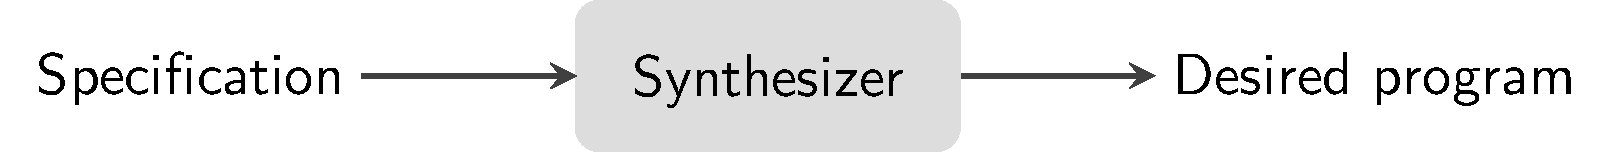
\includegraphics[scale=.35]{pictures/program_synthesis.pdf}
    \caption{Program Synthesis}
    \label{fig:program-synthesis}
\end{figure}
Program synthesis is the task of automatically generating a program that satisfies some desired behaviour expressed as a high-level specification~(see \autoref{fig:program-synthesis}).
This specification can range from a complete formal definition, such as a first-order formula \cite{DBLP:conf/ijcai/Green69,DBLP:conf/pldi/GulwaniJTV11}, to more ambiguous descriptions of the desired program's behaviour, like a set of input-output examples~\cite{balog2017deepcoder,DBLP:conf/pldi/FengMBD18,DBLP:conf/icse/JhaGST10,DBLP:conf/ijcai/ShawWG75,DBLP:journals/jacm/Summers77} or a natural language sentence~\cite{DBLP:conf/icse/DesaiGHJKMRR16,DBLP:journals/pacmpl/Yaghmazadeh0DD17}.

According to \citeauthor{PSnow}~\cite{DBLP:conf/ppdp/Gulwani10,PSnow}, a program synthesizer is typically characterised by three key dimensions:
\begin{enumerate*}[label=(\roman*)]
  \item the way the user specifies the desired characteristics of the program,
  \item the space of all possible programs the synthesizer can generate, and
  \item the search technique used to explore that space.
\end{enumerate*}

\paragraph{Desired behaviour specification} is the most important characteristic of a synthesizer from the users' point of view. It is the language in which they describe the behaviour of the program they intend to generate. It must take into consideration the underlying task, the users' technical background and which material is available when using the synthesizer.

\paragraph{Program space} is the set of all programs the synthesizer can possibly generate. In other words, it is the space over which the synthesizer searches for a feasible program. It depends on the domain of the problem the synthesizer is intended to solve. It must be expressive enough to ensure the desired program is included, but also restricted enough lest the search problem become intractable.

\paragraph{Search technique} refers to the method employed to find the desired program within the program space. It can be based on enumerative search, deductive search, constraint solving, or some combination thereof.

% \textcolor{purple}{It can be based on exhaustive search, version space algebras, machine learning techniques (such as belief propagation or genetic programming), or logical reasoning techniques.
% Most logical reasoning techniques involve two main steps: constraint generation, and constraint solving. (a) Constraint generation can be invariant-based, path-based, or input-based. (b) Constraint solving of resultant second-order quantified formulas typically involves reducing second-order unknowns to first-order unknowns (by use of templates), and eliminating universal quantifiers (by use of techniques such as Farkas lemma, cover algorithms, sampling), and then solving the resultant first-order quantifier-free constraints using off-the-shelf SAT/SMT solvers.}

\medskip

The three dimensions are further described in sections~\ref{sec:desired-behaviour-spec}, \ref{sec:program-space} and \ref{sec:search-technique}, respectively.

Program synthesis is a very wide field of research. It has been studied by different research communities and applied to diverse problems. As such, many approaches have been proposed to deal with the specific challenges introduced by each application, resulting in a great variety of focused algorithms that aim at finding a better program in less time. In this section, we take a more in-depth look into some of these techniques.

In \autoref{sec:cegis}, we look at a way to steer the search in the right direction by using information about wrong answers to avoid future similar mistakes. In sections~\ref{sec:ogis} and~\ref{sec:user-interaction}, we look at different ways to deal with the ambiguity of the desired behaviour specification in inductive synthesis.

Finally, in \autoref{sec:synth-predicates}, we take an in-depth look at \textit{AlphaRegex}, a tool that, though not directly addressing the form validation problem, tackles the synthesis of regular expressions, which are an important part of our domain.

\subsection{Desired Behaviour Specification} \label{sec:desired-behaviour-spec}
For the synthesis procedure to start, the user must first specify the program's intended behaviour. The desired behaviour can be described in many different ways, and is internally converted to some sort of behavioural constraints, which the output program must satisfy.

\begin{definition}[Desired Behaviour Specification]
The desired behaviour specification is a predicate \(\phi\), such that \(\phi(\vec{x}, y)\) is \true{} if and only if \(y\) is the desired output value for the input vector \(\vec{x}\).
\end{definition}


The first approaches to automating the creation of programs, proposed in \citeyear{DBLP:conf/ijcai/Green69} \cite{DBLP:conf/ijcai/Green69,DBLP:conf/ijcai/WaldingerL69}, were based in deductive synthesis.
Such synthesizers work based on a complete formal specification of the desired program's behaviour.
Then, they employ a theorem prover to construct a proof of the provided specification from which it is able to extract the executable program~\cite{DBLP:conf/ijcai/Green69,DBLP:journals/cacm/MannaW71,DBLP:journals/toplas/MannaW80,DBLP:conf/ijcai/WaldingerL69}.

Deductive synthesizers require the user to provide a complete formal description of the desired behaviour, such as a first-order formula.
Because it is a complete definition, the synthesizer always returns a program with the exact desired behaviour, and it is always satisfactory to the user.
However, writing these kind of specifications can be as complex as writing the program itself, and might force the user to learn a new formalism in any case.

\begin{figure}
    \centering
    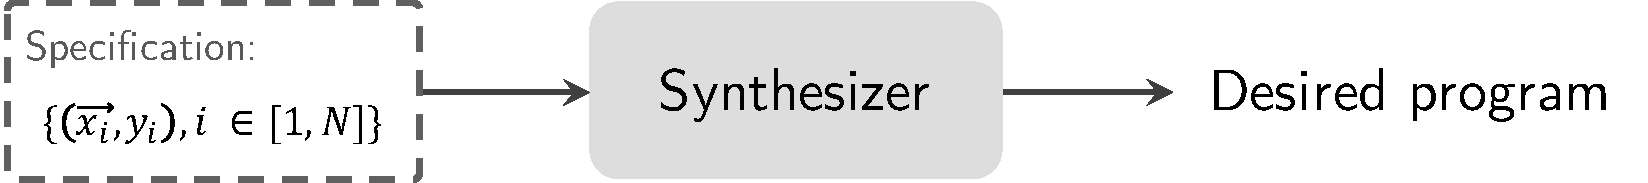
\includegraphics[scale=.35]{pictures/pbe.pdf}
    \caption{\ac{PBE}: The desired behaviour specification is a set of \(N\) input-output examples.}
    \label{fig:pbe}
\end{figure}

Such difficulties motivated a new approach to program synthesis: inductive synthesis \cite{DBLP:conf/pldi/FengMBD18,DBLP:conf/pldi/FengMGDC17,DBLP:conf/ijcai/ShawWG75,DBLP:journals/jacm/Summers77}. The program is then built based on simpler (albeit ambiguous) specifications, easier for the user to devise. \acf{PBE} is a branch of inductive synthesis where the user intent is specified using input-output examples~\cite{DBLP:conf/pldi/GodefroidT12,DBLP:conf/ijcai/ShawWG75,DBLP:journals/jacm/Summers77,DBLP:conf/sigmod/WangCB17,DBLP:conf/pldi/WangCB17}, as shown in \autoref{fig:pbe}.
%\textcolor{red}{(\cite{DBLP:conf/ijcai/ShawWG75} synthesises simple LISP programs from one input-output example.~\cite{DBLP:journals/jacm/Summers77} from several output examples)} or natural language descriptions~\cite{DBLP:conf/icse/DesaiGHJKMRR16}).

\begin{definition}[Input-Output Examples]
Input-output examples are a type of incomplete specification defined as a set of \(N\) tuples:  \(\mathcal{X} = \{(\vec{x_i}, y_i), i \in \{1, ..., N\}\}\) where each \(y_i\) is the desired return value for input \(\vec{x_i}\).
\end{definition}

\begin{definition}[\acl{PBE}]
Programming by example is the problem of synthesising a program using input-output examples as a specification of the desired program behaviour. In programming by example, the behavioural constraint is
\[\bigwedge_{(x_i, y_i) \in \mathcal{X}} P(x_i) = y_i,\]
which states that program \(P\) is correct if it yields the correct output for the inputs specified in the specification.
%\[\phi(\vec{x}, y) = \neg (\exists z : (\vec{x}, z) \in \{(\vec{x_i}, y_i), i \in \{1, ..., N\}\} \wedge z \neq y)\]
\end{definition}

\begin{comment}
\begin{example}
Suppose we would like to generate a function which, for any integer input numbers \(x_1\) and \(x_2\) returns their sum:
\[f(x_1, x_2) = x_1 + x_2\]
A \ac{PBE} synthesiser would require some input-output examples as input, for example:
\[\{((1, 1), 2), ((1, 0), 1), ((2, 1), 3), ((2, 0), 2), ((1, 2), 3)\}\]
\end{example}
\end{comment}


Input-output examples, although easier for the users to obtain and comprehend, are an incomplete specification. In general, there are several programs consistent with the provided specification even though not all of those correspond to the desired program and might not exhibit the behaviour expected by the user for cases that are not covered by the specification.

The ambiguity of input-output examples raises the necessity of selecting one among multiple candidate programs. One way to do this selection is by ranking the correct programs according to the measure of some characteristic that is desirable in programs of the domain in question, and returning to the user the program that ranks the highest.
Common desirable characteristics used to rank the programs include: execution speed (when we are looking for an efficient program), robustness (how well it generalises to new input-output examples), and readability (uses common operations in the underlying language making it easy for the user to understand).
Another approach is to enable the synthesizer to interact with the user to try and disambiguate the underlying intent. Section~\ref{sec:user-interaction} provides more details on this topic.

\subsection{Program Space} \label{sec:program-space}
The next step towards finding a program that satisfies the user's needs is defining the space of programs over which the synthesizer perfors the search: the program space.
We cannot consider all the programs that can be written using a full-featured programming language, as too many programs would be taken into consideration, rendering the search space intractable.
On that account, we need to restrict the language in which the programs are written in order to enable an efficient search of the program space.
However, we must ensure it remains expressive enough to capture many real-world tasks within the considered specialised domain.
We call this language \acf{DSL}.
The choice of a synthesizer's \ac{DSL} is crucial: it must allow a good balance between expressiveness and efficiency.

\begin{definition}[\acl{DSL}]
Domain specific language is the restricted language in which the synthesised programs are written. It includes information about both form (syntax) and meaning (semantics).
\end{definition}


One may impose restrictions on the allowed datatypes, as well as the operations over them so as to include only those relevant for the considered domain. For example, one could allow only integers and comparison operations, or arithmetic operations, or even only operations supported in some API exported by a given library. We can also restrict the program space by imposing constraints over the control structure of the program: we may disallow looping structures in the program, or bound the number of statements.

The constraints imposed on the language are named structural constraints, and they define the search space the synthesiser must consider. A \ac{CFG} is typically used to define the syntax of the \ac{DSL}.

\begin{definition}[Context-Free Grammar]
A \acl{CFG}~\cite{Jurafsky} is defined by a 4-tuple \((N, \Sigma, R, S)\), where:

\(N\) is a set of non-terminal symbols,

\(\Sigma\) is a set of terminal symbols (disjoint from \(N\)),

\(R\) is a set of rules or productions, each of the form \(A \to \beta\), where:

\quad \(A\) is a non-terminal,

\quad \(\beta\) is a string of symbols from the infinite set of strings \((\Sigma \cup N)*\), and

\(S\) is a designated start symbol and a member of \(N\).
\end{definition}


\acf{SyGuS} \cite{DBLP:conf/fmcad/AlurBJMRSSSTU13} is the branch of program synthesis in which the user to supplies the language syntax (in the form of a grammar) alongside the behaviour specification. This provides structure to the program space, which may allow for a more efficient search method. Furthermore, the generated programs are more interpretable to the user and better adapted to the domain at hand, since they are derived from the given grammar. On the other hand, \ac{SyGuS} requires the user to have a deeper technical knowledge not only on the specific domain on which he or she is working but also on formal languages and how to define them.

%Restricted DSLs can also enable more efficient special-purpose search algorithms. For example, if we consider a DSL that allows only the concatenation of substrings of an input string, a dynamic programming can be used to efficiently enumerate all possible outputs and thus search on such a space~\cite{DBLP:conf/oopsla/PolozovG15}.

% string programming/expression language that supports restricted forms of regular expressions, conditionals and loops. Expressive SQL queries

\subsection{Search Technique}\label{sec:search-technique}

Program synthesis can be seen as a search problem. It aims at finding a program in the search space defined by structural constraints that satisfies the behavioural constraints.

\begin{definition}[Program Synthesis]
Given a specification of desired behaviour \(\phi\), program synthesis is the problem of finding a program \(P\) that satisfies~\(\phi\).
\end{definition}


Several search techniques have been explored to solve program synthesis. In the remainder of this section, some of these search techniques are briefly explained. Note that one synthesizer does not have to apply only one of these techniques; more often, a combination of several techniques is applied.

\begin{figure}
    \centering
    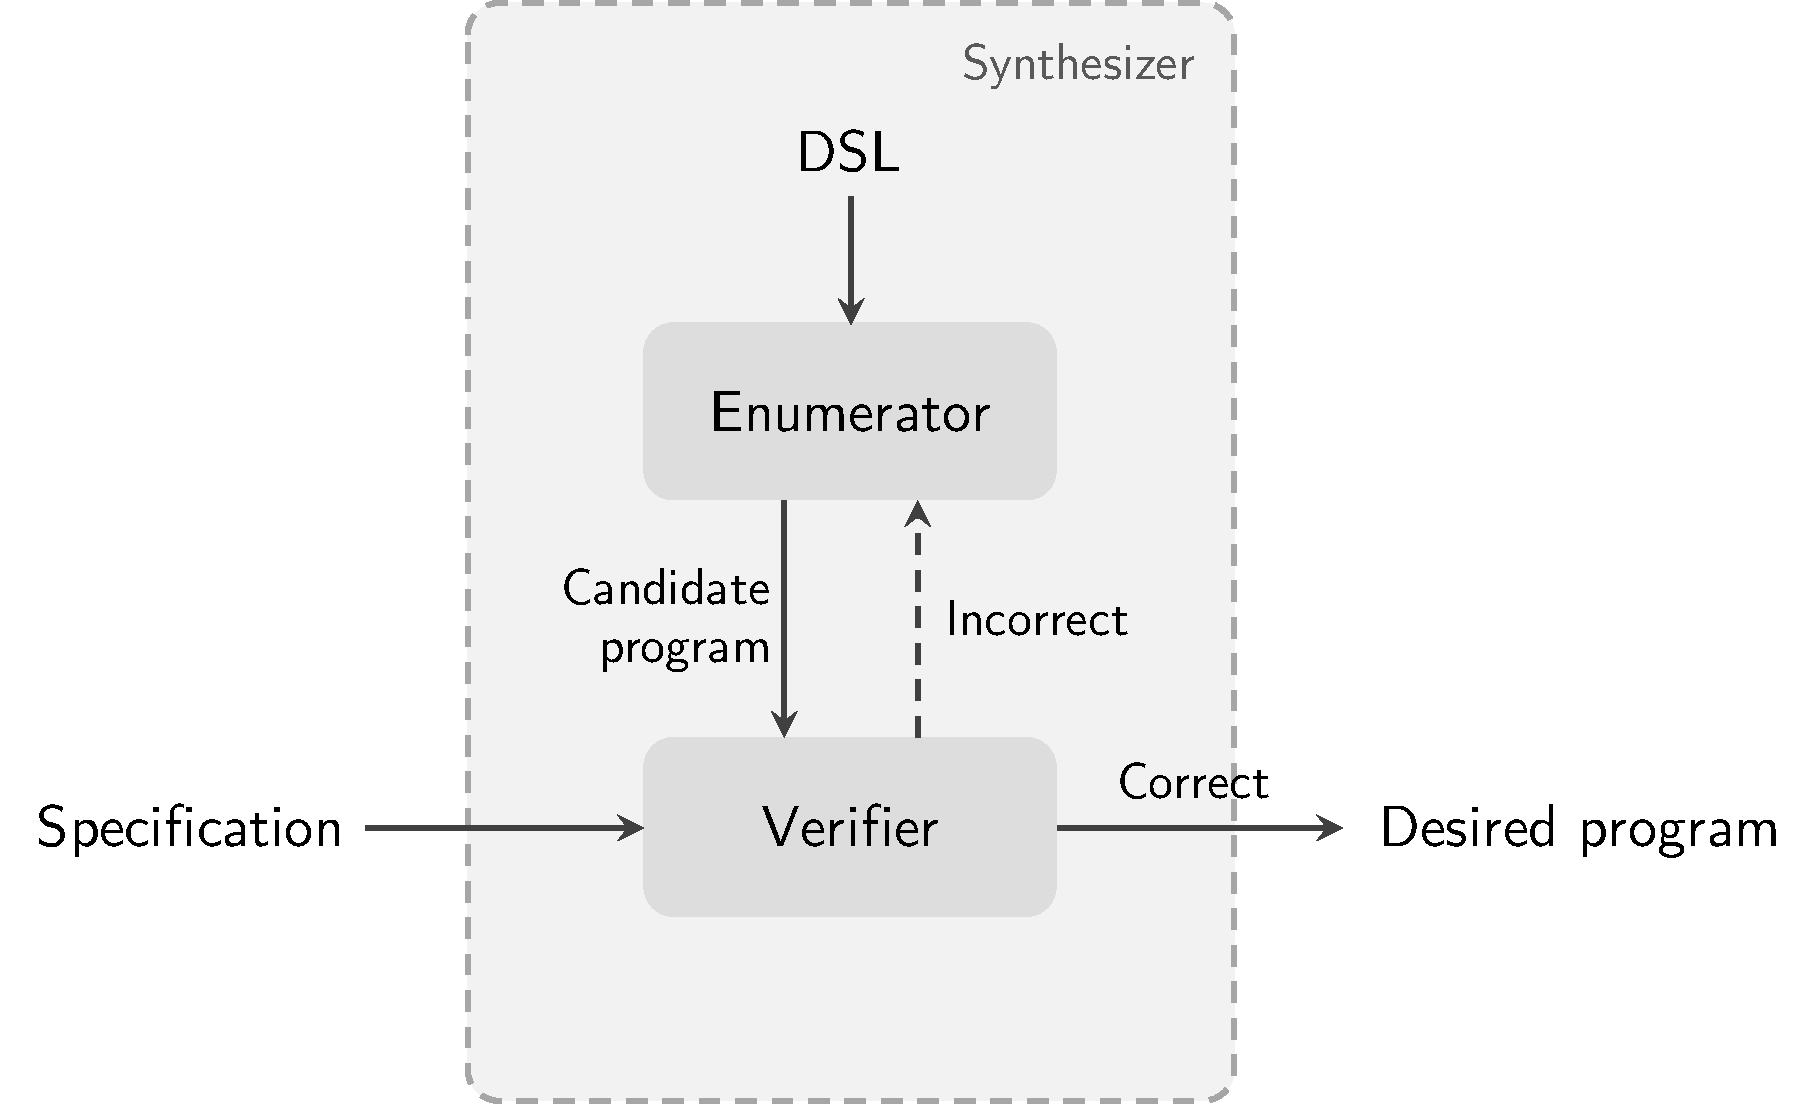
\includegraphics[scale=.35]{pictures/enumerative_search.pdf}
    \caption{Enumerative search}
    \label{fig:enumerative_search}
\end{figure}

\paragraph{Enumerative Search}\label{sec:enum-search}\cite{DBLP:conf/pldi/FengMGDC17,DBLP:conf/pldi/FengMBD18,DBLP:conf/gpce/LeeSO16,Orvalho19,DBLP:conf/cav/ReynoldsBNBT19} is a common approach to solve the search problem of program synthesis. In this technique, we have two key components: an \textit{enumerator} and a \textit{verifier}.
The \textit{enumerator} successively enumerates programs from the program space in some order. For each candidate program, the \textit{verifier} subsequently checks whether it satisfies all behavioural constraints, i.e., it is consistent with the user intent specification.
If the \textit{verifier} deems the program consistent with the given specification, then the program is correct and it can be returned to the user.
If, on the other hand, the \textit{verifier} decides that the given program does not satisfy the specification, then the \textit{enumerator} must pick a new program from the search space.
This loop is described in \autoref{fig:enumerative_search}.

A naive implementation of enumerative search does not scale to complex programs; however, it is a very effective strategy when coupled with some optimisation techniques. First off, the program space must be structured according to some metrics, usually program size or complexity, such that the \textit{enumerator} yields simpler programs first and only when those are refuted by the \textit{verifier} are more complex programs considered. This concept contributes to solving the problem of user intent ambiguity introduced in \autoref{sec:desired-behaviour-spec} by applying the Ockham's Razor principle: choose the simplest program that is consistent with the specification.

Another way to speed up enumerative search is by employing pruning techniques, such as discarding equivalent programs from the search space.
%The \textit{verifier} may also try to formulate a hint as to why a program deemed incorrect is not consistent with the specification and notify the \textit{enumerator}
In addition, when the \textit{verifier} rejects a program, it may apprise the \textit{enumerator} of the reason behind the program's incorrectness, thus reducing the program space and preventing the \textit{enumerator} from generating programs that fail in the same way.
This idea is further discussed in \autoref{sec:cegis}.

\paragraph{Deductive Search} \cite{DBLP:conf/oopsla/PolozovG15} is based on a top-down propagation of constraints through the grammar that defines the program space. It recursively reduces the problem of synthesising an expression that satisfies a certain specification to simpler sub-problems, thereupon combining those results.

Suppose we want to synthesise an expression \(e\) of the form \(F(e_1, e_2)\) that complies with a specification \(\phi\). Deductive search would leverage the inverse semantics of \(F\) to push constraints on \(e\) down through the grammar into constraints on \(e_1\) and \(e_2\). Finding \(e_1\) and \(e_2\) are then simpler sub-problems whose solutions, once found, can be combined to produce the originally desired expression \(e\).

Deductive search is very convenient when the underlying grammar allows for a rich set of constants. In such cases, enumerative search is no longer viable. A new enumeration step may be required for each possible constant in order to find the right one, resulting in too many iterations. On the other hand, the top-down deductive technique can deduce constants based on the accumulated constraints as the last  step in the search process.

\paragraph{Constraint Solving} \cite{Solar-LezamaPhDThesis,DBLP:conf/popl/SrivastavaGF10} consists on somehow generating a logical formula whose solution yields the intended program, and then solving it.

Several approaches can be used to generate the formula. On one extreme, we have invariant-based methods, which generate one formula that is satisfiable if and only if the program is consistent with the specification. Upon solving such a formula, we have not only a correct program but also a inductive proof of its correctness.
However, these methods do not scale well with the complexity of the specification --- the resulting formula may be intractable, and much more complex than the program itself.

To circumvent this drawback, we can instead make use of input-based methods. Then, the formula asserts the correctness of the program only on a subset of all possible inputs, which leads to much simpler constraints.

Once we have a logic formula, it must be solved. These formulas are of second-order logic, and need to be first reduced to first-order quantifier-free constraints that can the be solved using an off-the-shelf logic-based solver. Second-order reduction can be achieved using techniques such as \ac{CEGIS} \cite{Solar-LezamaPhDThesis}, which is described in \autoref{sec:cegis}.

\chapter{Related Work / Program Synthesis}

\section{Sketch-based Enumerative Search}
\begin{figure}
    \centering
    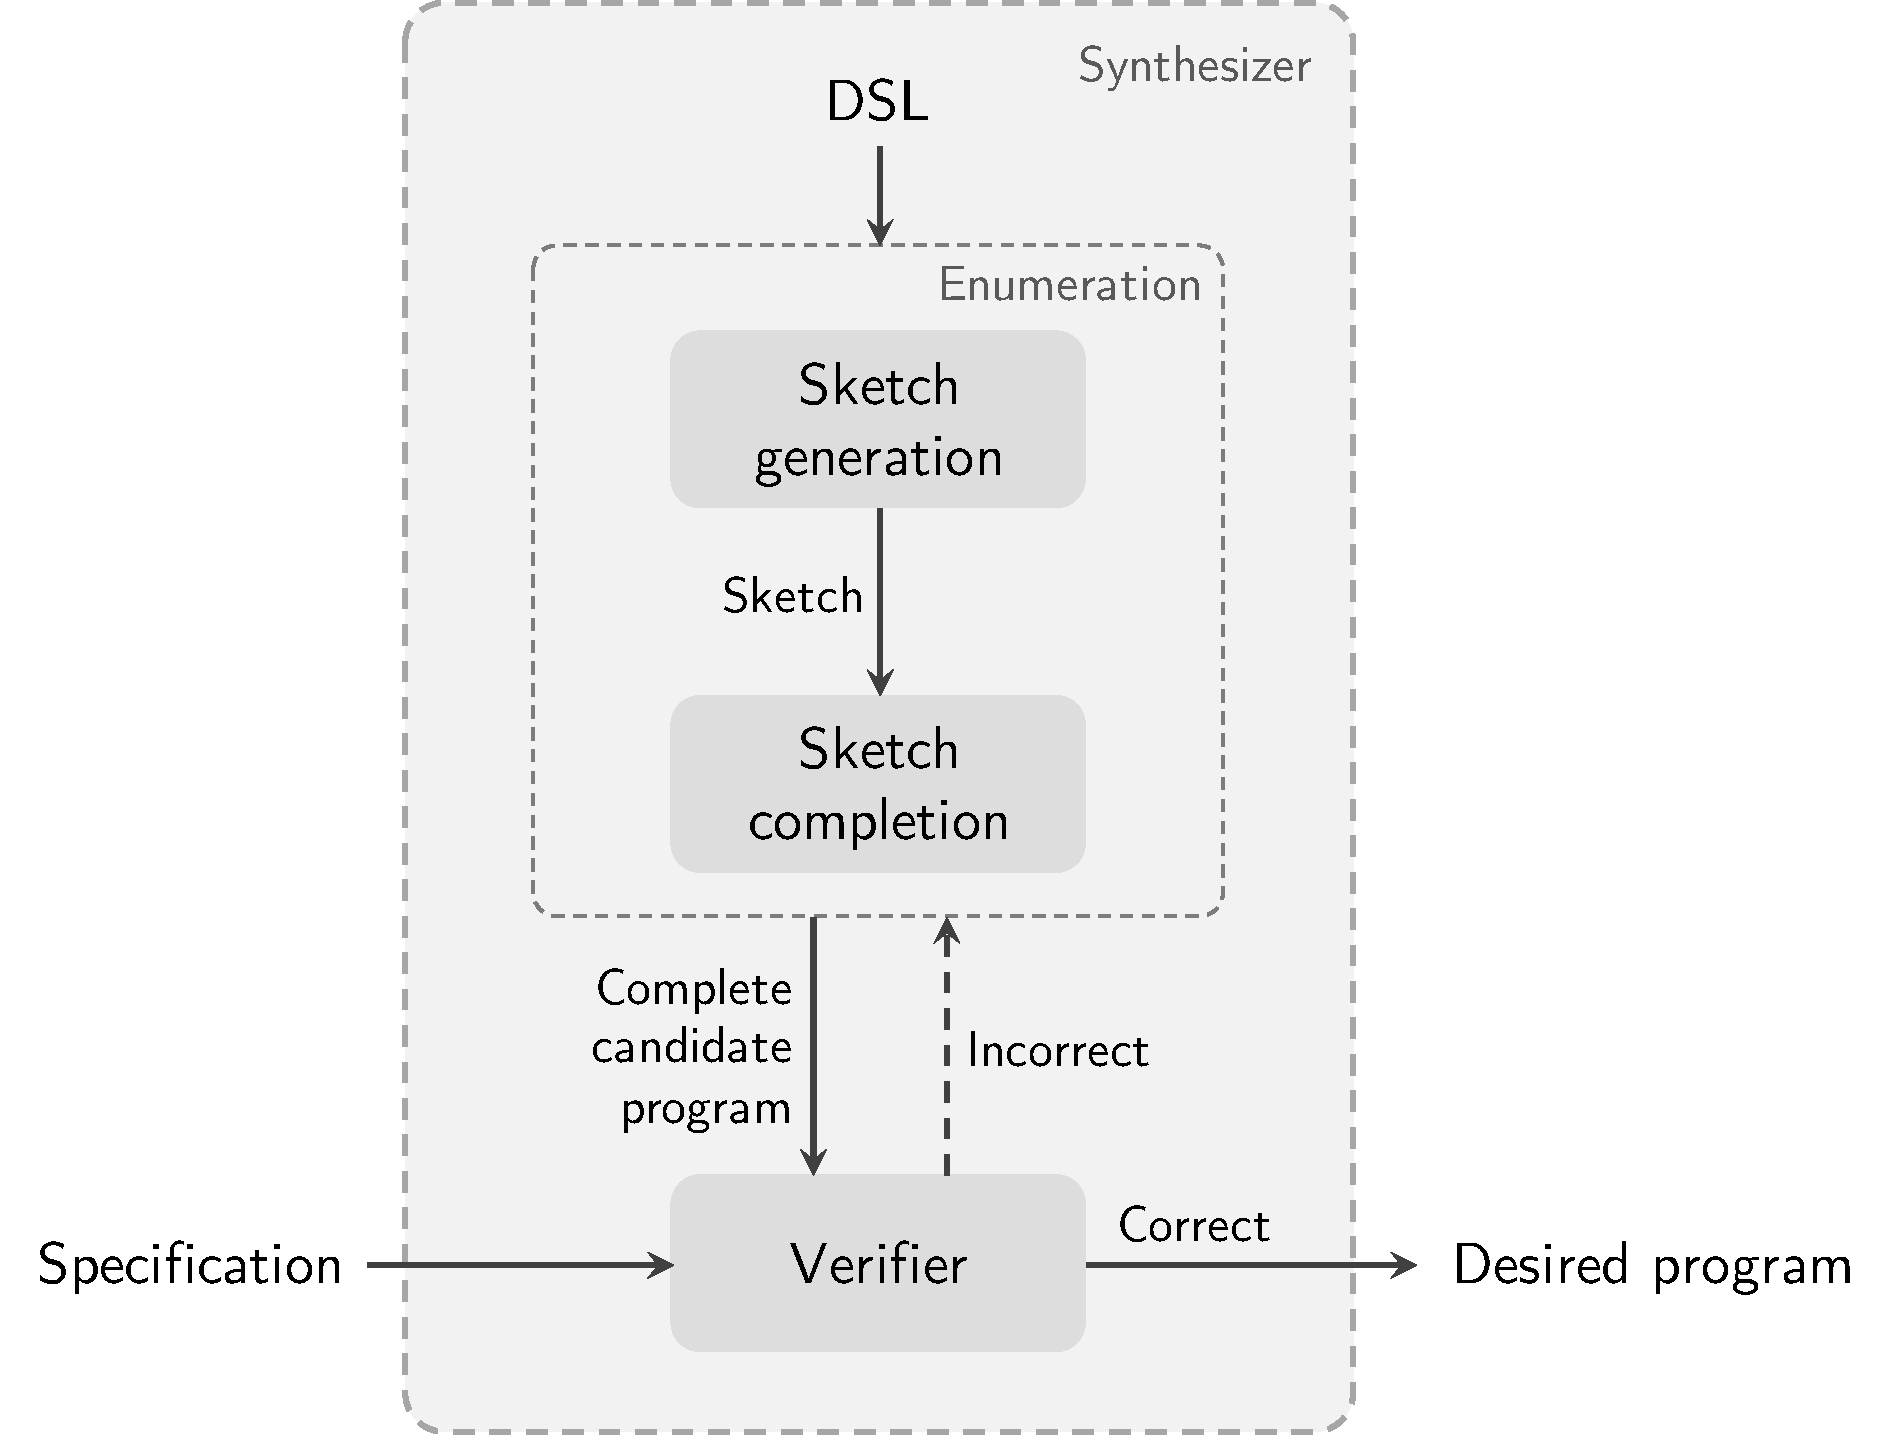
\includegraphics[scale=.35]{pictures/sketch.pdf}
    \caption{Sketch-based enumeration}
    \label{fig:sketch_enumeration}
\end{figure}
Some synthesizers opt to perform enumerative search using partial programs.
Partial programs (often called sketches) are a high-level representation of the intended program. Instead of completely defining a program, they contain holes, i.e., parts of the program that refer to lower-level implementation details. For a sketch to become syntactically correct, all its holes must be filled with syntactically correct expressions.

Instead of enumerating complete programs, a sketch-based synthesizer takes one of two approaches: Either
\begin{enumerate*}[label=(\roman*)]
    \item a sketch is provided by the user, who already possesses a high-level description of the desired program, in which case the synthesizer must complete it according to the specification, or
    \item the synthesizer is responsible for both producing a suitable sketch and completing it. The enumeration process is then split in two steps: sketch generation and sketch completion.
\end{enumerate*}
During sketch generation, the synthesizer enumerates incomplete programs in some order. During sketch completion, the synthesizer then enumerates complete programs for each given sketch, by successively filling each hole with a syntactically correct expression. Sketch-based enumeration is outlined in \autoref{fig:sketch_enumeration}.


\section{\acl{CEGIS}}\label{sec:cegis}

Program synthesis is a search problem where the goal is to find a program \(P\) that satisfies a given specification \(\phi\).
\(\phi(\vec{x}, y)\) is \true{} if and only if \(y\) is the desired output value for input \(\vec{x}\).
We can define the program synthesis problem with the following logic formula:
%
\begin{equation}\label{eq:ps-2nd-order}
\exists P \; \forall \vec{x}, y : (P(\vec{x}) = y) \Rightarrow \phi(\vec{x}, y).
\end{equation}
%
\noindent
Due to the existential quantifier over function \(P\), \eqref{eq:ps-2nd-order} is a second-order formula and, as such, it is generally undecidable. 
To work around this problem, we may note that even though \textit{finding} a program that satisfies a specification may be infeasible, \textit{verifying} that a given program \(P\) satisfies a specification is a first-order problem:
%
\begin{equation}\label{eq:ps-1st-order}
\forall \vec{x}, y : (P(\vec{x}) = y) \Rightarrow \phi(\vec{x}, y).
\end{equation}
%
Formula \eqref{eq:ps-1st-order} is a first-order formula and can be solved using an off-the-shelf first-order solver. Any program \(P\) that satisfies~\eqref{eq:ps-1st-order} is a correct program, i.e., it complies with the specification \(\phi\).
Instead of proving \eqref{eq:ps-1st-order}, we can equivalently disprove its negation:
%
\begin{equation}\label{eq:counterexample}
\exists \vec{x}, y : (P(\vec{x}) = y) \wedge \neg \phi(\vec{x}, y).
\end{equation}
%
Formula \eqref{eq:counterexample} is also a first-order formula.
Formula~\eqref{eq:counterexample} is unsatisfiable if and only if \(P\) is a correct program.
Therefore, to find a correct program, we search the program space for a program \(P\) such that~\eqref{eq:counterexample} is unsatisfiable. Once found, \(P\) can be returned to the~user. %To achieve this, we can use enumerative search (previously explained in \autoref{sec:enum-search}), whose definition fits well into this way of verifying correctness of the program: the \textit{verifier} entity is then a solver that tries to satisfy formula~\eqref{eq:counterexample} (see Figures \ref{fig:enumerative-search} and~\ref{fig:CEGIS}).

\begin{figure}
    \centering
    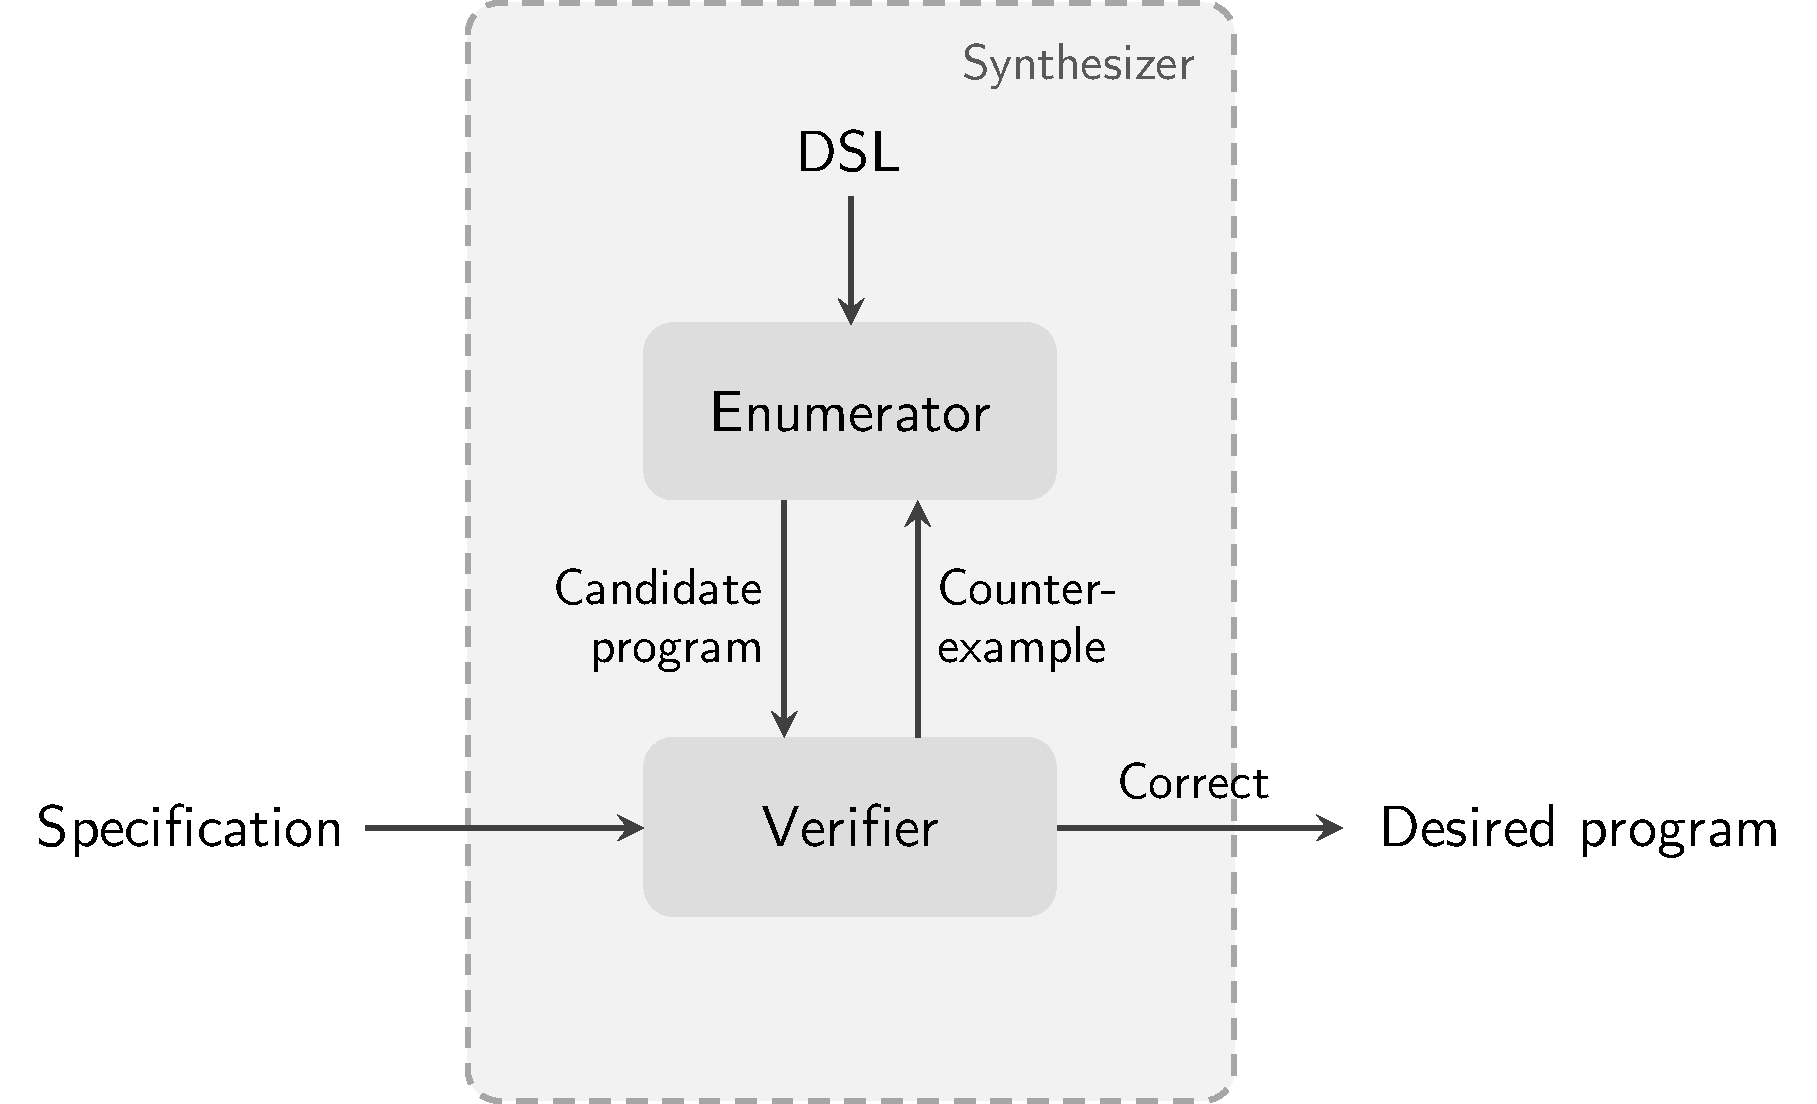
\includegraphics[scale=.35]{pictures/cegis.pdf}
    \caption{\ac{CEGIS}}
    \label{fig:cegis}
\end{figure}

Whenever we encounter a program \(P\) for which formula~\eqref{eq:counterexample} is satisfiable, the values of \(\vec{x}\) and \(y\) that satisfy the formula constitute a counterexample: an input \(\vec{x}\) for which \(P\) does not satisfy the specification \(\phi\); in other words, an input \(\vec{x}\) to which our program returns the wrong output.
If we take this counterexample \((\vec{x}, y)\) into account during our subsequent search, none of the new candidate programs will return \(y\) on the input \(\vec{x}\).
We have thus strengthened the specification, eliminating the previous incorrect candidate program.

\begin{definition}[Counterexample]
A counterexample \((\vec{x}, y)\) for an incorrect program \(P\) is an input-output pair such that \(P(x) = y\) and \(\neg \phi(\vec{x}, y)\), i.e., \(y\) is the output returned by \(P\) on input \(\vec{x}\) even though \((\vec{x}, y)\) is not consistent with the specification.
\end{definition}

This approach was proposed in \citeyear{Solar-LezamaPhDThesis} by \citeauthor{Solar-LezamaPhDThesis} in his PhD Thesis \cite{Solar-LezamaPhDThesis} and it is represented in \autoref{fig:cegis}. In this figure, the \textit{verifier} is a solver that tries to satisfy formula~(\ref{eq:counterexample}).

We can further improve this method by reformulating the verification formula in order to produce a constructive counterexample:
%
\begin{equation}\label{eq:constructive}
\exists \vec{x}, y : (P(\vec{x}) \neq y) \wedge \phi(\vec{x}, y).
\end{equation}
%
Like before, \eqref{eq:constructive} is a first-order formula and it is unsatisfiable if and only if \(P\) is a correct program.
When \eqref{eq:constructive} is satisfiable \(P\) is not a correct program and the values of \(\vec{x}\) and \(y\) that satisfy the formula are now a \textit{constructive} counterexample: \(y\) is the correct output for input \(\vec{x}\).
While a model \((\vec{x}, y)\) that satisfies \eqref{eq:counterexample} is an input-output pair that the program must \textit{not} satisfy, a model \((\vec{x}, y)\) that satisfies \eqref{eq:constructive} is a correct input-output pair that the program \textit{must} satisfy.
Adding the constructive counterexample to our previous specification results in a much stronger constraint and prunes the remaining search space even further. %However, this reformulation is only possible when there is only one output value that satisfies the specification for the input value~\(\vec{x}\).

\begin{definition}[Constructive counterexample]
A constructive counterexample \((\vec{x}, y)\) for an incorrect program \(P\) is an input-output pair such that {{\(P(x)~\neq~y\)}} and \(\phi(\vec{x}, y)\), i.e., \(y\) is not the output returned by \(P\) on input \(\vec{x}\) even though \((\vec{x}, y)\) is consistent with the specification.
\end{definition}

\section{\acl{OGIS}} \label{sec:ogis}
As discussed in \autoref{sec:desired-behaviour-spec}, \ac{PBE} comes with the drawback of incompleteness of the behaviour specification. Many programs are consistent with the provided specification, but not all these programs exhibit the user's intended behaviour.

In order to restore soundness of the solution, \citeauthor{DBLP:conf/icse/JhaGST10} proposed in \citeyear{DBLP:conf/icse/JhaGST10} a new approach which makes use of distinguishing inputs to disambiguate the input-output examples: \acf{OGIS}~\cite{DBLP:conf/icse/JhaGST10}.
An \textit{I/O~oracle} maps any given input to the desired output and it is used as an alternative to a complete specification. This means that whenever the \textit{I/O~oracle} is queried on any input vector \(\vec{x}\), it always returns the correct output \(y\).

We start with the same schema we had for \ac{CEGIS} (\autoref{fig:cegis}),  with a \textit{verifier} which, upon receiving a program \(P\), decides whether it is consistent with the behavioural constraints~\(\phi\). However, in \ac{OGIS} we no longer return to the user the first correct program we find.

When a correct program \(P_1\) is found, it is stored, and the search continues for another correct program. If no other correct program is found, then \(P_1\) is the unique correct program and it can be returned to the user. If another correct program \(P_2\) is found, then we have two programs consistent with the provided specification, i.e., \(P_1\) and \(P_2\) satisfy the following formulas:
%
\begin{subequations}
\begin{equation}
  \forall \vec{x}, y : (P_1(\vec{x}) = y) \Rightarrow \phi(\vec{x}, y),
\end{equation}
\begin{equation}
  \forall \vec{x}, y : (P_2(\vec{x}) = y) \Rightarrow \phi(\vec{x}, y).
\end{equation}
\end{subequations}

\noindent
Upon finding two correct programs, we want to find an input to which the two programs \(P_1\) and \(P_2\) return different outputs: a \textit{distinguishing input}. To produce a distinguishing input, we can try to solve:
%
\begin{equation}\label{eq:distinguishing}
  \exists \vec{x}, y_1, y_2: P_1(\vec{x}) = y_1 \wedge P_2(\vec{x}) = y_2 \wedge y_1 \neq y_2.
\end{equation}
%
If formula~(\ref{eq:distinguishing}) is unsatisfiable then \(P_1\) and \(P_2\) are equivalent programs.
In this case, either there are more correct programs that can be taken into consideration, or \(P_1 = P_2\) is the unique program that satisfies all input-output examples and it is returned to the user.
If~(\ref{eq:distinguishing}) is satisfiable, the distinguishing input \(\vec{x}\) can be extracted from the model \((\vec{x}, y_1, y_2)\) that satisfies it.
Once found, we can query the \textit{I/O oracle} on the distinguishing input, who yields the correct output for it.
The distinguishing input along with its correct output forms a new correct input-output pair \((\vec{x}, y)\) which can then be added to the specification~\(\phi\), further constraining the search space.

In the end of this cycle, we have a set of input-output pairs that completely specify the generated program, thus eliminating all ambiguity.

\begin{figure}
    \centering
    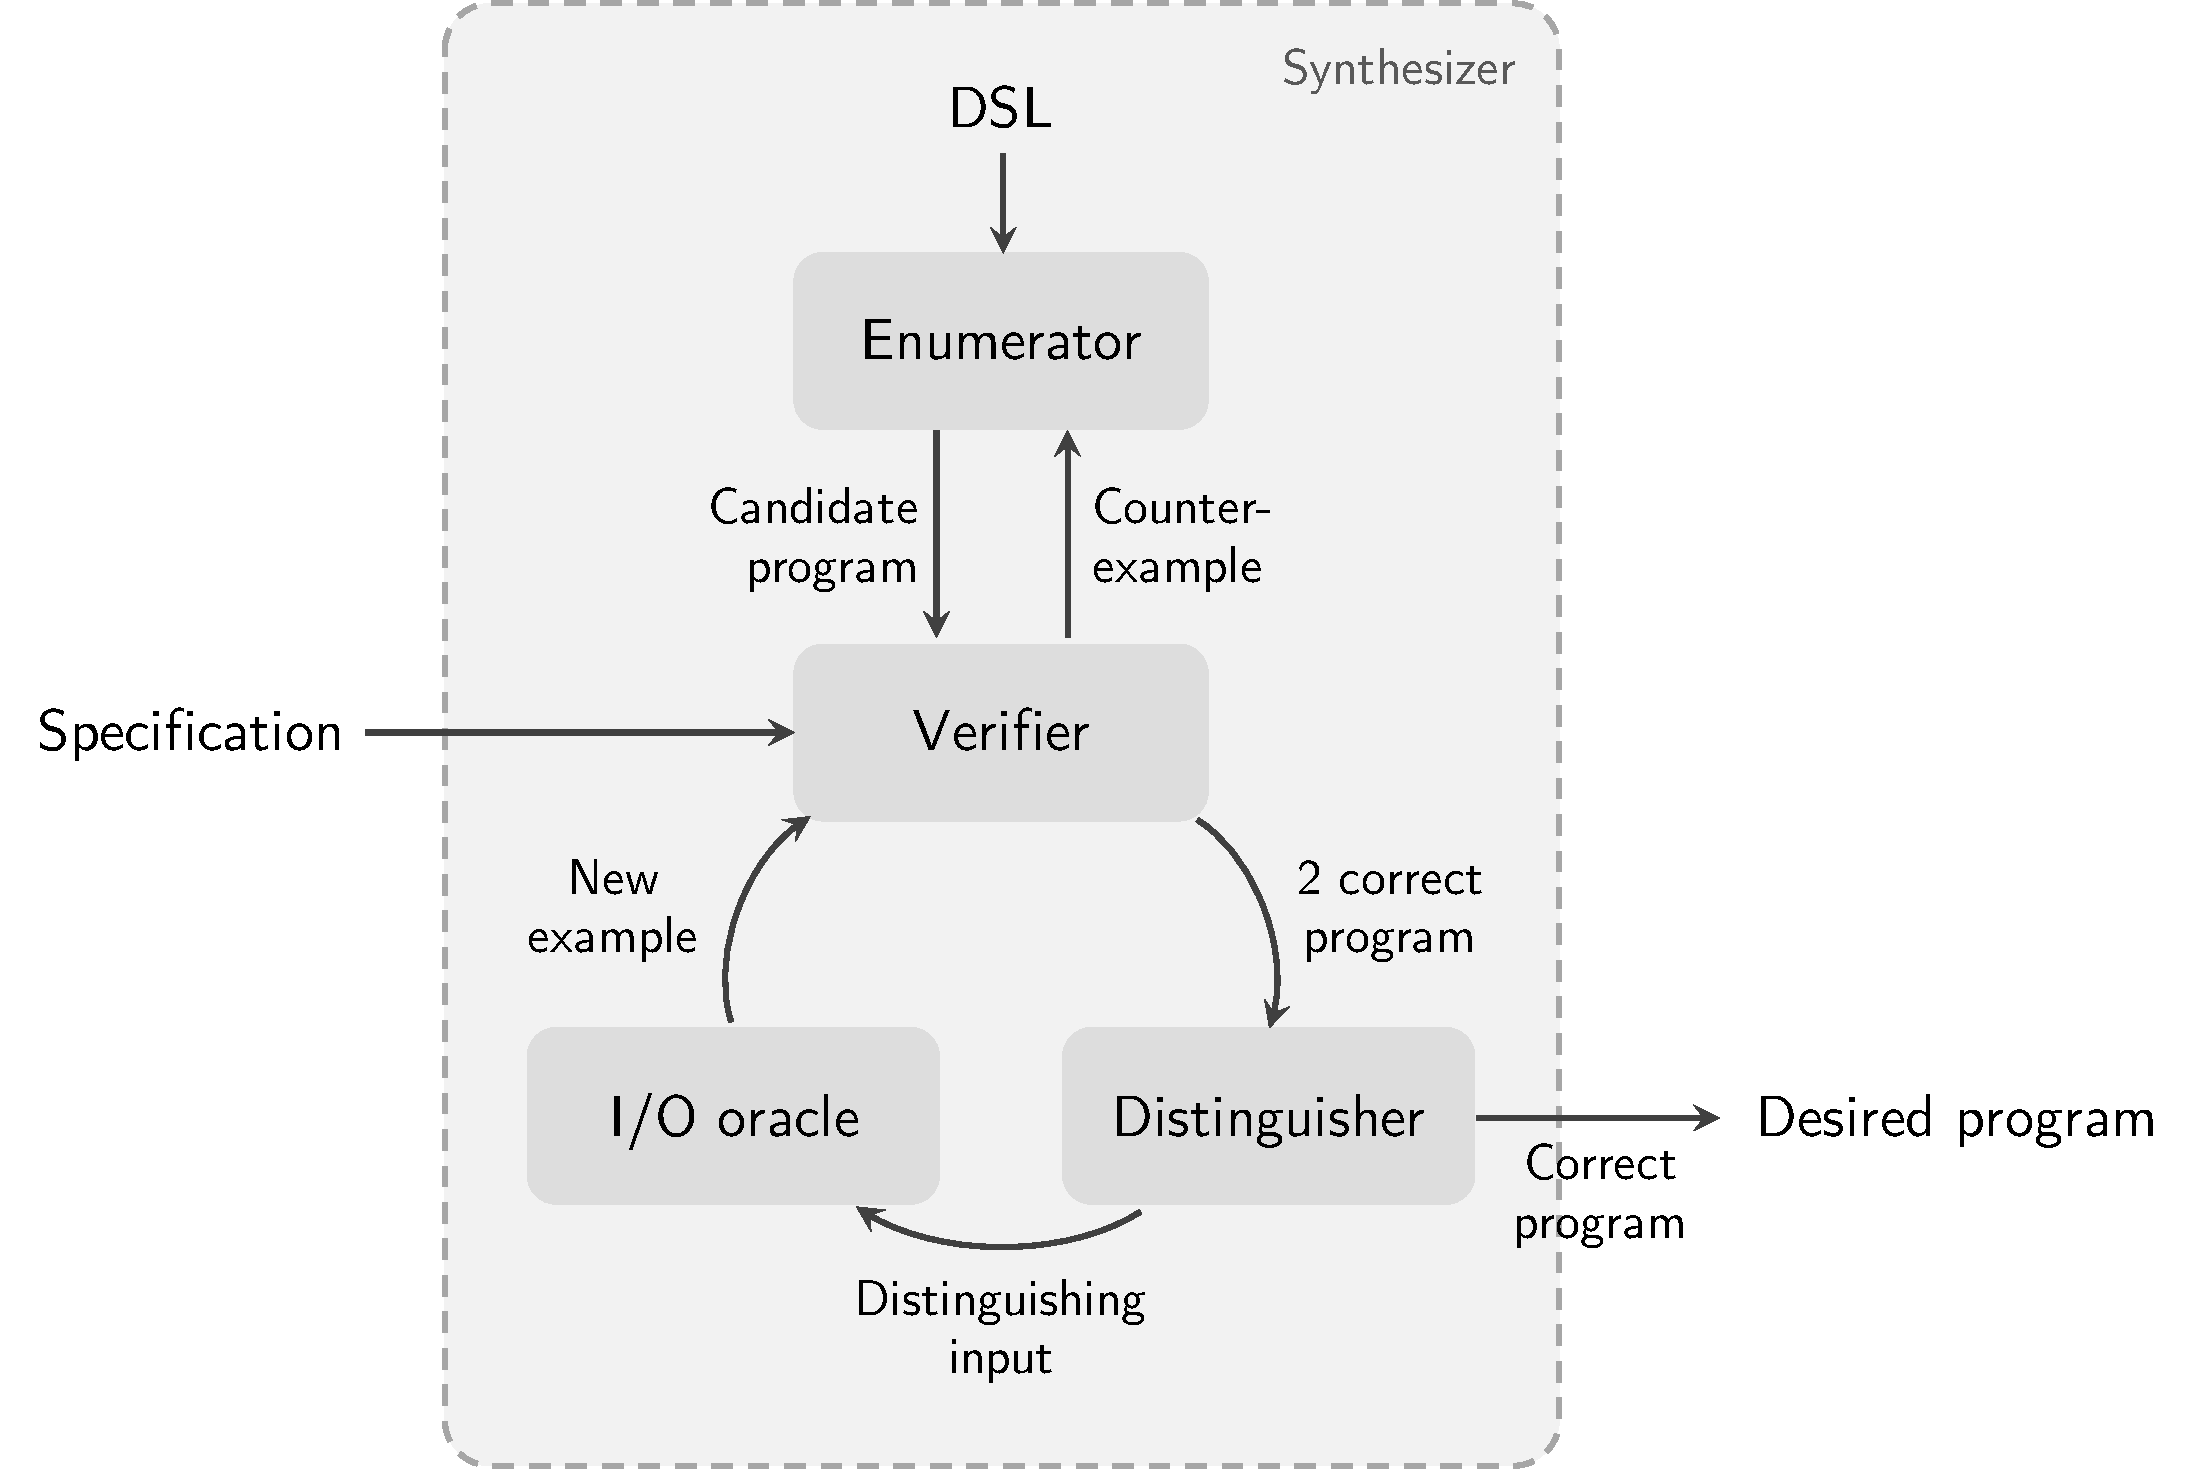
\includegraphics[scale=.35]{pictures/ogis.pdf}
    \caption{\ac{OGIS}}
    \label{fig:ogis}
\end{figure}

This method is illustrated in \autoref{fig:ogis}. In this figure, the \textit{enumerator} and \textit{verifier} are identical to those in \ac{CEGIS} (\autoref{fig:cegis}). The \textit{distinguisher} is a new entity, which can be a solver that tries to satisfy formula~(\ref{eq:distinguishing}).


\section{User Interaction} \label{sec:user-interaction}

As mentioned before, \ac{PBE} uses input-output examples as the desired behaviour specification, which can be very ambiguous. When the synthesizer simply picks a correct program to return to the user, it may not satisfy the desired behaviour in corner cases not covered by the examples provided.
In order to increase confidence in the synthesizer's solution, a good way to disambiguate the specification is by explicitly interacting with the user so he or she can provide further information about the intended~program.
% In this section we look at two different user interaction models that allow the synthesizer to gather more information about the intended program, thus resolving the ambiguity in the initially provided examples.

\subsection{Conversational Clarification}
\begin{figure}
    \centering
    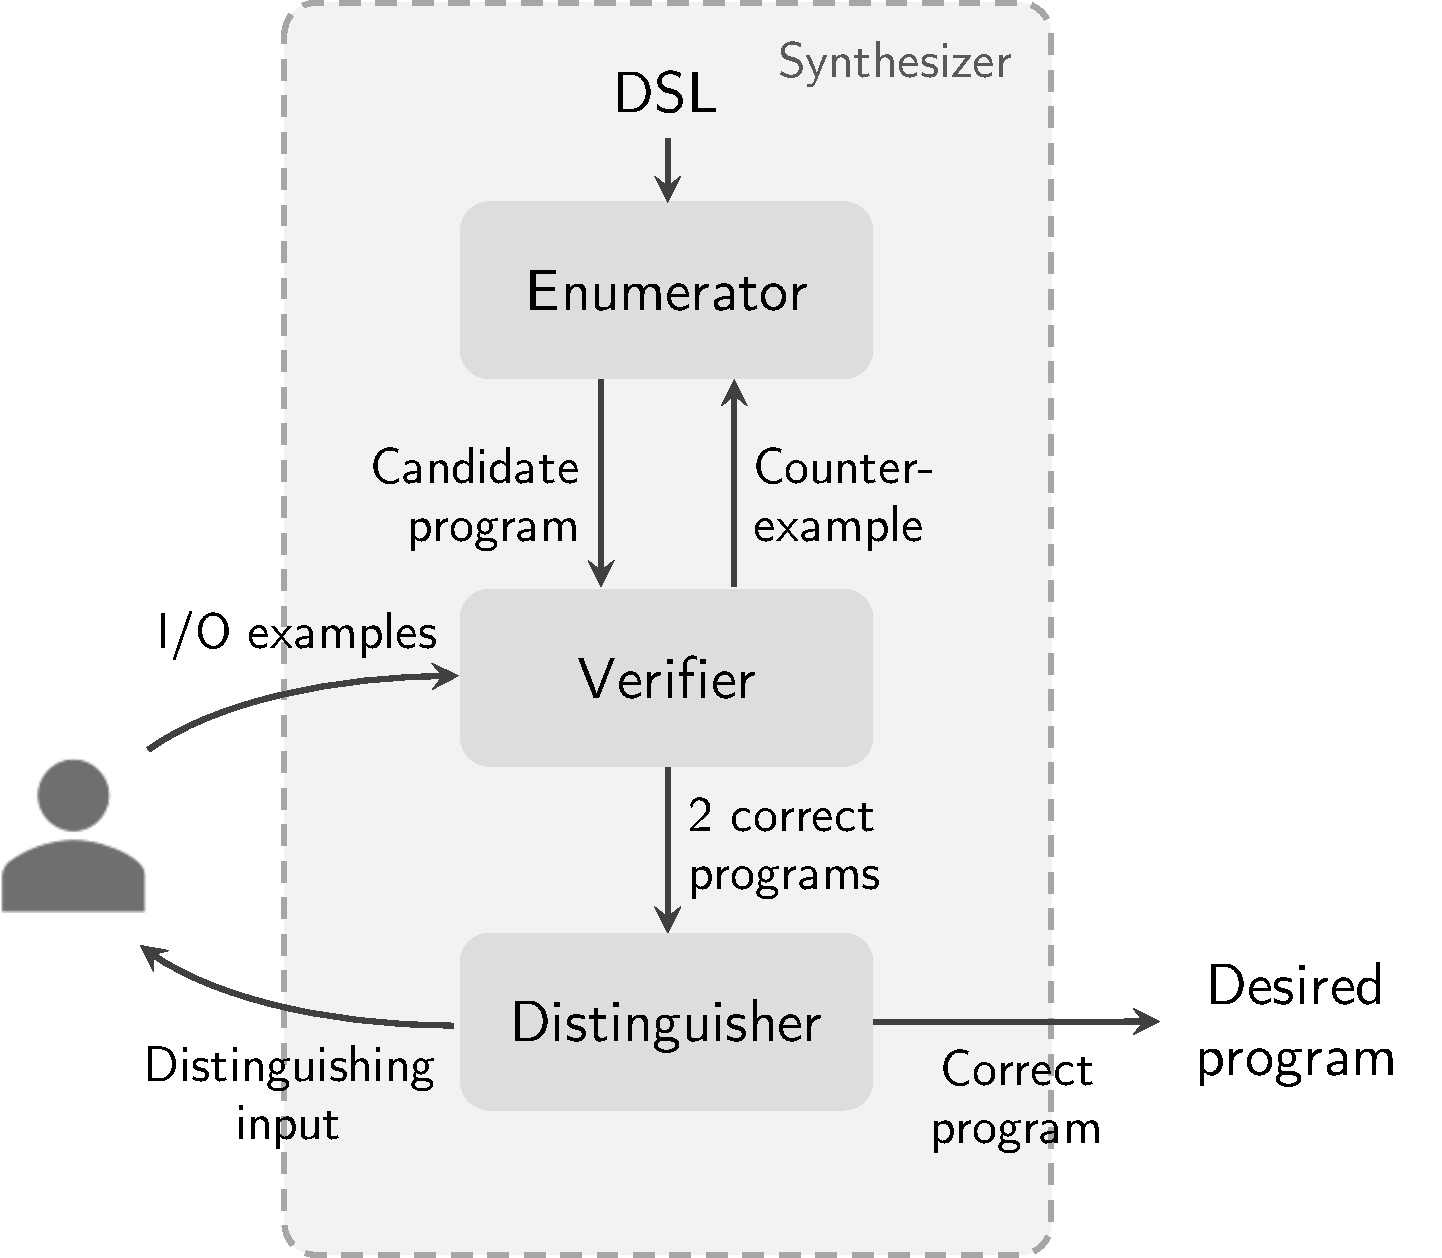
\includegraphics[scale=.35]{pictures/conversational_clarification.pdf}
    \caption{Conversational clarification}
    \label{fig:conversational_clarification}
\end{figure}

Conversational clarification is an interaction method described by \citeauthor{DBLP:conf/uist/MayerSGLMPSZG15} \cite{DBLP:conf/uist/MayerSGLMPSZG15} which has been successfully used in many synthesizers  \cite{DBLP:journals/pvldb/LiCM15,DBLP:journals/corr/abs-19,DBLP:conf/sigmod/WangCB17,DBLP:conf/pldi/WangCB17}.
During the synthesis procedure, the synthesiser asks questions to the user with respect to certain inputs, and uses the answers to resolve ambiguities in the desired behaviour specification. 

After the synthesizer has generated several programs that are consistent with the user-provided examples, it uses the \textit{distinguisher} described in \autoref{sec:ogis} to produce a distinguishing input: an input for which two correct programs yield two different outputs. The synthesizer then queries the user on what is the desired output for that specific input (it may be the output returned by one of the synthesised programs, or a different one altogether). The distinguishing input along with the desired output form a new input-output example, which is added to the specification, making it stronger. Each distinguishing input splits the search space in a different way, so the number of necessary user interactions depends on the chosen distinguishing input in each iteration. In the end, only one program remains. Since all ambiguity in the original specification has been resolved, the remaining program is the desired program and it can be returned to the user.

Conversational clarification is represented in \autoref{fig:conversational_clarification}. It is no more than a variation of the \ac{OGIS} method, described in \autoref{sec:ogis}, where the user plays the part of the \textit{I/O oracle}.


\subsection{Ramos's Interaction Models}

\citet{UnchartIt} propose two interaction models: \textsc{Options} and Y/N. Both models interact with the user using distinguishing inputs, i.e., new inputs generated by the synthesizer that allow

\section{Regex synthesizers}\label{sec:related-work}



\subsection{\textit{AlphaRegex}}
\label{sec:synth-predicates}
In \citeyear{DBLP:conf/gpce/LeeSO16}, \citeauthor{DBLP:conf/gpce/LeeSO16} \cite{DBLP:conf/gpce/LeeSO16} presented \textit{AlphaRegex}, a \ac{PBE} synthesizer of regular expressions in the binary alphabet, \(\Sigma = \{0, 1\}\).

To use \textit{AlphaRegex}, the user describes the desired accepted language by providing a set of positive and negative examples. The synthesised regular expression must define a language that includes all the positive examples and none of the negative ones.
\textit{AlphaRegex} uses an enumerative search technique, with a ranking method that prioritises simpler expressions.

The algorithm starts by examining the simplest regular expressions, \regex{0} and \regex{1}.
If these are not consistent with the examples, it checks more complex productions such as \regex{0|0}, \regex{0|1}, \regex{1|0}, \regex{1|1} (i.e. expressions in the form of \regex{\Box|\Box}), \regex{00}, \regex{01}, \regex{10}, \regex{11} (i.e. expressions in the form of \(\tt\Box\Box\)), and \regex{0*}, \regex{1*}, (i.e. expressions in the form of \(\tt\Box*\)).

Here, we introduce the hole (\(\Box\)), a placeholder for any regular expression. Regular expressions with or without holes are the states of the search.
The algorithm generates regular expressions by iteratively replacing holes with other states and checking if the resulting regular expressions are correct.

To speed up the search, \textit{AlphaRegex} makes use of three different kinds of search space pruning techniques: over-approximation, under-approximation and elimination of redundant states.

\paragraph{Over-approximation} is achieved by replacing holes in the current state with \regex{(0|1)*}.
This regular expression describes the language that accepts all the strings that can be written using the binary alphabet.
%The union of any  regular expression \(r\) with \regex{(0|1)*}, \(r|\tt(0|1)*\), is again \regex{(0|1)*}.
%The concatenation of any regular expression \(r\) with \regex{(0|1)*}, \(r\tt(0|1)*\), results in the original regular expression \(r\).
Therefore, over-approximation makes the state as general as it can be.
If the over-approximation rejects at least one of the positive examples we conclude that this state can never be used to build a solution.

\begin{example}
Consider the state \(\tt1\Box\), i.e., the concatenation of \regex{1} with a hole, which can be filled with any regular expression. The over-approximation of this state, \regex{1(0|1)*}, accepts all strings that a regular expression of the form \(\tt1\Box\) could possibly accept. Thus, if \regex{1(0|1)*} does not accept all the the positive examples, this state is not worth considering, and can be pruned.
\end{example}

\paragraph{Under-approximation} consists in replacing holes in the current state with \regex{\emptyset}, the regular expression that corresponds to the empty language. The concatenation of any regular expression \(r\) with \(\tt\emptyset\), \(r\tt\emptyset\), results in \(\tt\emptyset\). The union of any  regular expression \(r\) with \(\tt\emptyset\), \(r|\tt\emptyset\), is the regular expression \(r\) itself.
If the under-approximation does not reject any of the negative examples,  we conclude that this state can never be used to build a correct solution.

\begin{example}
Consider now the state \(\tt1|\Box\), i.e., the union of \regex{1} with a hole. The under-approximation of this state, \(\tt1|\emptyset = 1\), restricts \regex{1|\Box} to the language that accepts as few strings as possible, in this case, the one containing only the string with a single `1'. If \regex{1} does not reject any of the negative examples, then this state can be pruned.
\end{example}

\paragraph{Elimination of redundant states} is done using the equivalences of regular expressions resulting from the algebraic rules of regular expressions.
%  described in \autoref{tab:regex-laws} in \autoref{sec:regex}
For example, the algorithm needs not evaluate the expression \(s\texttt{|}r\) if it has already considered \(r\texttt{|}s\), where \(r\) and \(s\) are regular expressions, as these expressions are equivalent.

\medskip

\noindent
The authors tested \textit{AlphaRegex} in 25 benchmark problems collected from textbooks on automata theory which are provided along with the code for their tool.
\textit{AlphaRegex} proved capable of synthesising relatively complex expressions, with more than a dozen operations, in under one minute.


\subsection{\textsc{Regel}}